\documentclass[epsf]{article}
\usepackage{amsmath,amsthm,amsfonts,latexsym,amscd, framed}
\usepackage{graphicx}

\textwidth=6.0truein\hoffset=-.5truein
\textheight=8.5truein\voffset=-.5truein

\begin{document}
%\maketitle
\newcommand{\R}{\mathbb{R}}
\newcommand{\noi}{\noindent}
\newcommand{\bs}{\bigskip}

%%%%

\begin{center}
{\Large Project \#4: Phase Portraits for Linear DE Systems\\
\vskip 2mm
Pre-Work}
\end{center}


\noi{\bf PW 1} Choose the phase portrait (on the next page) that corresponds to each the following DE systems.  As you are thinking about the problems, take notes on why you chose or ruled out a certain phase portrait.  You can use your notes from section to help you write justifications for your choices on the solutions page for DP\#4.

\begin{itemize}
\item[(a)] The system $\vec{\bf x}' = \begin{bmatrix}-1 & 1\cr\ \ 0 & 1 \end{bmatrix}\vec{\bf x}$ has general solution
$\vec{\bf x}(t) = c_1e^{-t}\begin{bmatrix}1 \cr0 \end{bmatrix} + c_2e^{t}\begin{bmatrix} 1 \cr 2 \end{bmatrix}$.

\noi NOTES:

\vskip 1.3 in

\item[(b)]  The system $\vec{\bf x}' = \begin{bmatrix}2 & 2\cr 1 & 3 \end{bmatrix}\vec{\bf x}$ has general solution
$\vec{\bf x}(t) = c_1e^{4t}\begin{bmatrix}1 \cr1 \end{bmatrix} + c_2e^{t}\begin{bmatrix} -2 \cr \ \ 1 \end{bmatrix}$.

\noi NOTES:

\vskip 1.3 in

\item[(c)] The system $\vec{\bf x}' = \begin{bmatrix}0 & -2\cr 2 & \ \ 0 \end{bmatrix}\vec{\bf x}$ has general solution
$\vec{\bf x}(t) = c_1\begin{bmatrix}-\sin(2t) \cr \cos(2t) \end{bmatrix} + c_2\begin{bmatrix}\cos(2t)\cr \sin(2t) \end{bmatrix}$.

\noi NOTES:

\vskip 1.3 in


\item[(d)] The system $\vec{\bf x}' = \begin{bmatrix}-1 & \ \ 1\cr -2 & -1 \end{bmatrix}\vec{\bf x}$ has general solution
$\vec{\bf x}(t) = c_1e^{-t}\begin{bmatrix}\sin(\sqrt{2}t) \cr\sqrt{2} \cos(\sqrt{2}t) \end{bmatrix} + c_2e^{-t}\begin{bmatrix}-\cos(\sqrt{2}t)\cr \sqrt{2}\sin(\sqrt{2}t) \end{bmatrix}$.

\noi NOTES:


\end{itemize}

\newpage

Each of the following is a phase portrait for a $2\times 2$ linear DE system. \\


\begin{center}
A 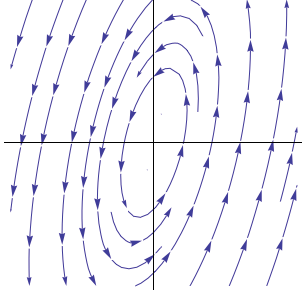
\includegraphics[width=40mm]{center1.png}\hspace{0.6 cm}B 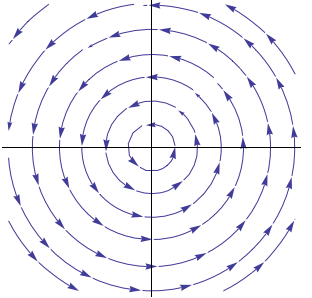
\includegraphics[width=40mm]{center2.png}\hspace{0.6cm}C 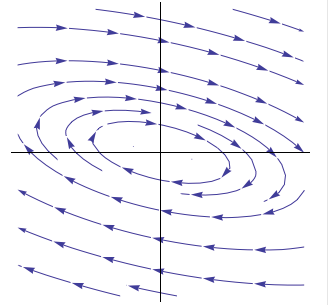
\includegraphics[width=40mm]{center3.png}\\

\vskip 1cm
D 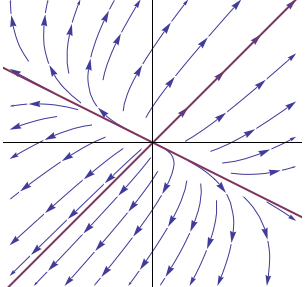
\includegraphics[width=40mm]{source1.png}\hspace{0.6 cm} E 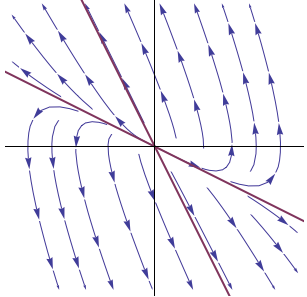
\includegraphics[width=40mm]{source2.png}\hspace{0.6 cm} F 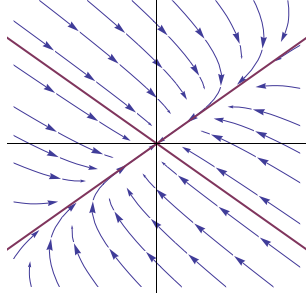
\includegraphics[width=40mm]{sink.png}\\
\vskip 1cm
G 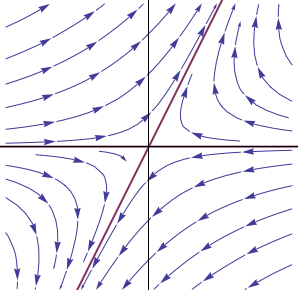
\includegraphics[width=40mm]{saddle.png}\hspace{0.6 cm} H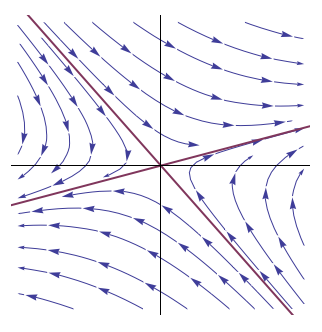
\includegraphics[width=40mm]{saddle2.png}\hspace{0.6 cm} I 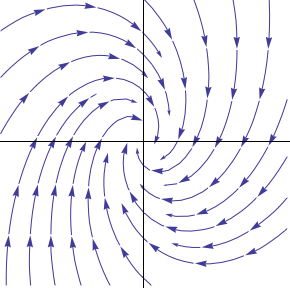
\includegraphics[width=40mm]{stable_spiral.png}\\
\vskip 1cm
J 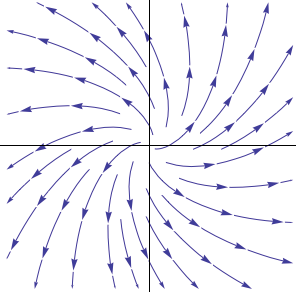
\includegraphics[width=40mm]{spiral_source.png}\hspace{0.6 cm} K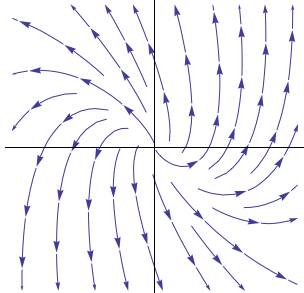
\includegraphics[width=40mm]{spiral_source2.png}\hspace{0.6 cm} L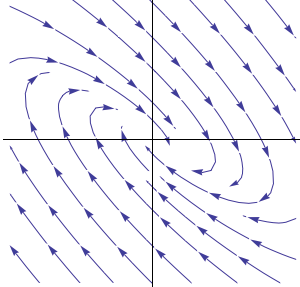
\includegraphics[width=40mm]{stable_spiral2.png}\\
\end{center}

\end{document}